\documentclass[twoside, 11pt]{scrartcl}

%%%%% General information %%%%%
\title{Overview Over My Bachelor's Thesis}
\author{Jannis Eichborn}

%%%%%%%%%% PACKAGES %%%%%%%%%%%
% basic packages
\usepackage[english]{babel}
\usepackage[utf8]{inputenc}
%\usepackage{cite}
\usepackage[sort]{natbib}
\usepackage{hyperref}
\usepackage{color}
%\usepackage{float}
\usepackage{graphicx}
\usepackage{floatrow}
%\usepackage{showframe}
\usepackage{fancyhdr}

%%%%%%%%%% SETTINGS %%%%%%%%%%%
% No indents, should be unchecked later
%\setlength{\parindent}{0pt}  

% make links in the document interactive
\hypersetup{linktoc=all}
\hypersetup{
    colorlinks,
    citecolor=black,
    filecolor=black,
    linkcolor=black,
    urlcolor=black
}

% Set the style of the header and the footer
\pagestyle{fancy}
\fancyhf{}
\fancyhead[LE,RO]{ }
\fancyhead[RE,LO]{\leftmark}
\fancyfoot[CE,CO]{}
\fancyfoot[RE,LO]{\thepage}
\renewcommand{\headrulewidth}{0.5pt}

% set the style for floating figures
%\floatstyle{boxed}
%\restylefloat{figure}

%%%%%%%%%% NEW FUNCTIONS AND DEFS %%%%%%%%%%%
\def\code#1{\texttt{#1}}

    


%%%%%%%%%%%%%%%%%%%%%%%%%%%%%%%%%%%%%%%%%%%%%%%%%%%%%%%
%%%%%%%%%%%%%%%%%%%%%%%%%%%%%%%%%%%%%%%%%%%%%%%%%%%%%%%
% The actual work
%%%%%%%%%%%%%%%%%%%%%%%%%%%%%%%%%%%%%%%%%%%%%%%%%%%%%%%
%%%%%%%%%%%%%%%%%%%%%%%%%%%%%%%%%%%%%%%%%%%%%%%%%%%%%%%
\begin{document}



\begin{titlepage}
\maketitle
%\textcolor{red}{*Things related to Usability later in the explanations}
\tableofcontents
\end{titlepage}

%%%%%%%%%%%%%%%%%%%%%%%%%%%%%%%%%%%%%%%%%%%%%%%%%%%%%%%
% Introduction
\section{Introduction \& Motivation}
\label{sec:introduction}
The motivation for the project described in this thesis stems from work in open-source communities and the development of a new programming language called \textit{Julia}. This chapter will talk about experiences and observations which led to idea of an online-database for the language Julia. It also introduces notations and related work.
%%%%%%%%%%%%%%%%%%%%%%%%%%%%%%%%%%%%%%%%%%%%%%%%%%%%%%%
\subsection{The current Open-Source Environment}
Working together on software has always been challenging already on company-wide scales.  In the movement of open-source communities sharing, reusing and distribution of code is an even bigger challenge and poses obstacles to the development of ideas still to this day. There are several approaches and with the rise of git-based systems there seems to be a clear favorite. But for some tasks in mind this may not be an optimal approach.\\

\textbf{Brief Description and History}\\
Open Source should be considered one of the biggest buzzwords in software-design of the 21st century. The way code is developed, people work together and the software is distributed is in constant change for the last 15 years. TODO find a source to give basis to these propositions.\\

The idea of sharing code over a largely distributed network of engineers existed before the Open-Source movement of today. It makes more sense to see it as an ongoing development which was dramatically enhanced with the spread of high-speed internet connections.(TODO something about Richard Stolzmann here!). One of the biggest achievements coming from the early community is the Unix operating system together with its childen Linux, Debian and other distributions.
These project are hugely complex in terms of time that was put in it, the amount of code produced, the number of collaborators and the spread of usage over the globe (TODO some kind of numbers would be nice for that, also I want to include something which shows the role of the internet in this development, what happened when and where, how were people connected while doing it?).

With the rise of the internet people began to pool their knowledge and skills in ways which were not possible a couple of years earlier. Programmers began, often in their free time, to input ideas, implementations and critics into open projects which did not earn them any money. Actually very often the licenses used prohibit any commercial use of the created programs as does, for example, the popular Apache license one can see in many Open-Source projectsTODO LINK.

Why would people do that?
Well there are two often named reasons for that. First of all the free software, where free does not only mean gratis but free of commercial interests has a strong ideological background from  people writing and using the programs. It is believed that if only enough people give to the community it will be self-sustaining and makes everyone actually profit from it in their creation of programs. 

Secondly, and more recently, people do it for actual credit. They will not be payed for their efforts directly but their efforts and input are visible to many people. A Developer makes contacts, generates a reputation and gains credibility which in the end enhances chances for better positions in profit-generating companies. In addition to that many of the quick-paced upcoming start-ups which have changed the software-landscape in the last years rely on the use of open-source technology. They constitute moving parts of a bigger system. MySQL is one example of a widespread open-source project in commercial use.

So the community began to grow quite quickly and it did not take too	 long until people began to have troubles working together on code. Keeping track of versions, contributions, contributors, bugs, milestones and many more is a challenge already with a couple of people sitting in the same room. Having code written by thousands of developers all over the world then, is a whole different story (TODO find a  source for the development of the linux kernel and the number of contributors).

\textbf{The Open-Source Community is Changing}\\
What are recent developments, how is code shared, where do we want to go?
Which ideals are fulfilled and which  things are still in a messy state?\\

\textbf{What is the Problem with Current Integrated Development Environments?}\\
Introduction of usability in the context of working with IDEs\\
Description of problems in the workflow regarding spreading of code, packages in different forms and finding suitable discussion and documentation. Reuse of code is bad and tedious.


\subsection{Our Idea for Working on Large Projects in the Future}
Description of the idea of having more code in one place with interchangeable and competing solutions. Using crowd sourcing for evaluation...\\
How is the functionality of an online database for code integral part of the IDE's usability?\\

\subsection{My Work \& Goals - A Self-organizing Database for Code}
What exactly will my work do in this context and what are my goals. 
Description of the structure of my thesis. What usability criteria do I aim for?\\

\subsection*{General notes - Abbreviations.}
\begin{itemize}
	\item I will use the term \textit{function} for anything that is a function, method, routine or subroutine in a given language. Maybe just talking about Julia here?
\end{itemize}



%%%%%%%%%%%%%%%%%%%%%%%%%%%%%%%%%%%%%%%%%%%%%%%%%%%%%%%
% Analysis and Formalisation of the Problem
\section{Analysis \& Formalisation}
\label{sec:analysis}
This chapter will present the considerations which are necessary to formalize the idea in order to design the system. The user or client, which in this case could also be another program,  is in the focus of attention in the analysis of requirements. These requirements then generate technical requirements which will be analyzed as well.
%%%%%%%%%%%%%%%%%%%%%%%%%%%%%%%%%%%%%%%%%%%%%%%%%%%%%%%

\subsection{Description of Use-Cases - Client Requirements}
\label{sec:clientReq}
\textit{This part will include extensive formalisations with respect to usability. How can this be formalised, what metrics can be derived? How do I define the client in this scenario and what is important to this client?\\
I describe how people are going to use the client IDE and what requirements arise from this. I will talk about portability between different OSs, what performance clients want and other aspects which are important to the implementation. What are possible interfaces and how can I meet them?}

% General thoughts
First of all I will have to describe potential clients to my system. What kind of applications will make use of the database, how do they want to communicate and what does this interaction imply for the architecture of the database?

Well to begin with is should be obvious, that I will not be concerned with any kind of graphical interface to the database. It would store millions of entries with several different versions of each entry. Of course one could think of means to make an interactive query interface which can display the database in it entirety but in my mind this is no use case. Users should always query the database in the context of a more elaborate system on top. If you wanted to search for documentation or code only there are already thousands of possibilities to do so on the internet (TODO quote).
From my point of view the system is designed to be used by an IDE or something equivalent. It does not mean that other more 'traditional' use-cases are not possible, but I will not be concerned with those in this chapter. Also the aimed database-representation would probably perform suboptimal for these kind of uses (multiple rapid queries at a time over simple indices). For these tasks there are solutions (TODO quote) out there and they cannot be the target use-cases for my system.

% Example in an IDE
In my mind the focus of the system must be to aggregate over the contained data for more elaborate queries. For example a query in plain English would be something like this: "Give me all the function signatures which match this given set of parameters" or "Which functions have the same parameters and return the same type?".\\
These queries result from using the a possible IDE or smart query system on top of the database. Let me stick with using an IDE for a more extensive example: A User writes a function from the top of his head. He does not refer to anything in the database (yet), but instead simply writes ahead. \\
Right after he has entered the signature the system can check for the following: 
\begin{enumerate}
	\item Is there already a function with the exact \emph{same signature}?\\
Should definitely be shown to the user. Maybe somebody has already done all the work he is going to do now. This might even be an expert in this area who has spend approximately 42 hours upon perfecting the runtime-behavior of this single function. In this case users might be happy to just plug-in the given function as is, or at least make use of the code to get ideas for his own improvements. I think this case might sound pretty uncommon but with thousands of users which roughly confirm to naming-standards of functions, this feature might work pretty fine right out of the box. Also users could then go ahead and write their own variants of this function an re-upload it. This way entering the desired signature alone can be seen as a means to search for functionalities using all the knowledge that you put into the signature.

	\item Is there already a function with the \emph{same name}?\\
Even if the signature is no a match, there might still be quite a lot of use in showing functions which have the same name. They might be different approaches to the same functionality - variations in the parameters might just be due to implementation details - or functions which are similar in their behavior and might need only slight changes to fulfil a new role. As it is the intention to make code reusable and having the database managing all the (sometimes rivalling) code-fragments.

	\item Is there already a function with a very \emph{similar name}?\\
Using some sort of similarity-measure, one could determine a class of function names which are similar enough to the given function name. Best case this is done using the general naming conventions of the language in question. There are two cases that are worthwhile to consider:
	\begin{enumerate}
		\item Are the parameters the same?\\
Then it is most propable that the user will want to see these results. There is quite a lot of information already in the typed parameter to a function. If those correspond it is worth a look to see whether this function might actually what the user wants in this context.
		\item Are the parameters - while not the same - at least similar\\
If the parameters are completely different it will be highly unlikely that the function will do what the user wants to achieve. If however the parameters differ only marginally it might be interesting to see also these function in the database.
	\end{enumerate}
\end{enumerate}

In general this all means that the database must be able to process these kinds of queries with reasonable results for all the given cases. While case 1) seems pretty straightforward, there might be problems when it comes to versioning of code pieces and finding the "best" functions which have the same signature. It is of no use for the user to find himself confronted with more than a dozen nightly-hacked matrix multiplications before the "standard" built-in matrix-multiplication is shown. \\
For all cases in 2) and 3) there is some sort of ranking necessary to present the client with usable results. Also one must consider, that you don't ever want to return \emph{all} results as bandwidth would quickly become a limiting factor to the system, which makes ranking even more interesting.
The system should make use of as much context-information as necessary, even drop down to comments in order to rank functions for a given query.\\

\textbf{Possible queries}
\begin{itemize}
	\item Retrieval of functions:
	\begin{itemize}
		\item Finding matching code to  a signature.(might also include the return type of the function)
		\item Find code to similar signatures or even without a name at all, just so you can see what would be possible with a set of arguments.
		\item Finding matching code to a block of code. (Potentially hazardous)
		\item Retrieving a newer version of code (maybe just the difference)
		\item Retrieving a whole package/module with all functions
		\item Retrieving meta-information to functions. Documentation, connections to other code, dependencies/using/requirements, variations, older version etc... 
		\end{itemize}
	\item Uploading functions:
	\begin{itemize}
		\item A completely new function, without any links. 
		\item Upload an entire module/package
		\item An update/extension to a function which the user wrote
		\item A variant to a function.
		\item Comments to a function
		\item A rating for a function
		\item A connection between code 
	\end{itemize}		
\end{itemize}

	 

\textbf{Defining the desired experience from a client's point of view}
\begin{itemize}
	\item Most obviously: Having a consistent, simple and well documented interface to the database. It is well defined what queries can be made (and how, maybe using DTD) as well as what one can expect as a response to those queries.
	\item The most important criteria: Having fast response times for simple queries (meaning super-fast retrieval of single functions). Searches for larger sets should yield responses quickly as well. Initial guess less than 500ms for first results to arrive.
	\item Finding the most current version of a function
	\item Finding the most relevant function if there are multiple implementations
	\item If one searches for a set of functions or if a query has mutliple matching results, the client will expect some kind of order on the results. This order should feel natural and consistent as people have become used to by modern search engines. If the database fails to deliever at this level people are far less likely to interact with the code and make updates to the system. 
	\item Up to this point I do not want to aim for auto-completion. The client should provide one query and expect a timely answer to it (no streaming yet). Later this feature might get interesting, especially once the database gets partitioned over several clusters and results are aggregated from different sub-graphs. For now my goal will be batched processing of one query after the other.
	\item Having consistent results. The same query deliveres the same answers, similar queries lead to similar results. Priorization should be transparent to a client, or even configurable (using some sort of arguments for a search).
	\item If a client updates information in the database or uploads new content, he will want to get feedback whether this was successful or not. Some auxiliary information might be interesting (what version, where, what size, how long etc...). If the transaction failed for whatever reason the client wants to know why.
\end{itemize}

\textbf{Required funtionalities derived from the desired experience and possible queries}
\begin{itemize}
	\item Fast (indexed) access to the data in various forms:
		\begin{itemize}
			\item function-names (some intelligent search like elastic search to be able to find similar names)
			\item parameters (in combination with the name or without it)
			\item return types in combination with the above.
			\item metainformation (not a priority)
		\end{itemize}		 
	\item Using these finding mechanism the database must be able to return:\
	\begin{itemize}
		\item A whole function, if there is exactly one hit, in a protocolled and serialized manner.
		\item Requested parts of functions (comments, ratings, documentation)
		\item Being able to traverse the graph in order to find connections (versions, similar functions, parameters, usage links etc...). \textbf{This functionalality is very interesting but is also vast and sometimes difficult. Thus it is not a priority.}
	\end{itemize}
	\item Also the database must return sets of functions:
	\begin{itemize}
		\item If a client wants to see/retrieve a package.
		\item If a client searches functions similar to a given signature.
		\item If a client only provides parameters and wants to find matching functions.
	\end{itemize}
\end{itemize}


\subsection{Non-functional (technical) Requirements to the System}
This section focuses on things like scalability, robustness, the iteration speed of changes, whether and where changes to the design are possible and how security and safety standards can or have to be met. Which things are necessary and which ones are nice to have?\\

\textbf{Building an interface}\\
The first task is to provide the functionality of the database-system to a remote client. There must be a suitable protocol in place which can handle the transfer or queries and the responses. Criteria: Quick, secure, fail-safe, well-known and understood. The datastream needed should be minimal to avoid loss of data as well as reducing the time/bandwidth needed for the transactions. A client should be able to use the system without a top-notch internet connection.\\



\textbf{Trying to minimize the time needed for the queries}\\
This is a central requirement.. Making data accessible is what the database is all about. The client-acceptance of the system is dependent on quick response of the system. Having a neat interface (above) is the first step. Furthermore the system must exhibitthe following properties, which I will explain below:
\begin{enumerate}
	\item Consistency of the data in order to keep the amount of space needed for the data minimal.
	\item Monitoring as a means to detect failures and bottlenecks in the system.
	\item Scalability.
	\item Ranking of results.
	\item Feedback when things timeout or fail.
\end{enumerate}


\textbf{1) Consistency of the data}
\begin{itemize}
	\item Being able to produce a \emph{unique} ID for every entry which encodes name, signature and timestamp for the given function which was uploaded. This ID must be unique for every entry but still encode in an understandable manner. A function can be translated to an ID and it must be possible to retrieve a function from an ID. (Indexing or traversals) 
	\item The database needs a valid scheme which represents structures in the data. Since I will use a graph-based system there has to be a graph-representation of the data, which is extendable and concise at the same time in order to prevent overhead in the data-representation while still having the means to extends functionalities in the system.
	\item Items which are put into the database have to be addressable, properly connected and indexed, so that there is no zombie-data in the database. Transactions need to be atomic for retries, dispatchement over different threads and support of thousands of clients. 
	\item One very important aspect is proper versioning of functions. Initially the database should be able to store as many version as the user likes. Over time it could be interesting to implement some garbage collection behavior to sort out unused nodes in the database to prevent the system from becoming overloaded in slow. There must be some way to monitor this behavior.
	\item Having a proper indexing system.
\end{itemize}

\textbf{2) Monitoring}\\
In order to assess the functionality of the database there have to be mechanism to generate and use simple metrics over the system. These metrics can then be used to optimize the behavior of the graph and to evaluate the success of different functionalities. Possible metrics are:
\begin{itemize}
	\item Number of transactions per second.
	\item Overall size of the graph; number of nodes/edges.
	\item Average number of connections between nodes. Distribution of types of connections.
	\item Average number of versions for one function (or other means of central tendency).
	\item How the client-access is distributed, how many calls of what category?
	\item Average times for operations.
	\item Error counts, failure statistics.
\end{itemize}


\textbf{3) Scalability}
\begin{itemize}
	\item The performance of the database must be consistent with growing input. One cannot assume constant behavior but linear would already be pretty bad. Mechanisms must be in place which allow efficient indexing and sorting of data.	
	\item Vertical scalability: If a machine has more resources it should be able to make use of those. More cores mean more threads. Atomic transactions have to be distributed over all available threads using the  provided memory in the heap. That means the database will have to be designed for heavy concurrency in all possible places (reading, writing, garbage collection, metrics).
	\item Horizontal scalability: With more and more data it is vital to be able to partition the data over multiple machines/drives. This should be considered from the start. The database should never be a monolithic process in a single JVM, or at least it must be possible to change that without rewriting the whole codebase. This includes considerations about the consistency of the data over multiple instances or partitions.
\end{itemize}

\textbf{4) Ranking of results} \\
\begin{itemize}
	\item Using some metrics to cap the search-space and the amount of data which has to be retrieved.
	\item This also means not to squander with the number of individual transactions (possibly concurrent) to the database, but to make processing batched. This will help serving a lot of clients while still providing fast answering to every one of them.
	\item There has to be a good understanding of the use-cases and distribution of usage to tune this system. Therefore the initial capabilities will be limited to rudimentary features.
\end{itemize}
  

\subsection{Goals of my Work}
Which derive from the requirements above. Explicit goals with respect to usability.


\subsection{Structure of My Work}
What comes first. How do I want to accomplish the goals and what is the prioritization.


%%%%%%%%%%%%%%%%%%%%%%%%%%%%%%%%%%%%%%%%%%%%%%%%%%%%%%%
% Relevant Basics
\section{Relevant Basics}
\label{sec:basics}
This section will introduce concepts which are essential to the general design of the software as well as the concrete implementation. One key concern is how  data can be stored such that the framework can perform the most occurring requests efficiently. A basis should be provided which is referred to in section \ref{sec:implementation} \textit{Implementation \& Design} . One aspect analyzed as well is the usability of the system to possible clients. This chapter will include some theoretic background and notations to the said aspects which will be used to assess the performance of a running prototype in a meaningful way. 
%%%%%%%%%%%%%%%%%%%%%%%%%%%%%%%%%%%%%%%%%%%%%%%%%%%%%%%
\subsection{JVM - Choice of Language and Context}
\label{sec:jvm}
Why it is still relevant in the context of large-scale distributed computation
\subsection{SQL to NoSQL - Why Graph Databases?}
What are recent developments in the requirements on databases and how are those met. New types of databases are emerging.
\subsection{Distributed Databases}
Distributed computations require new forms of data-management. Distributed systems lead to more scalability and robustness in the case of hardware-failures.
\subsection{General Thoughts on Performance \& Scalability in Recent Software Design}
What is the bottleneck in performance nowadays, how is that important to me.

\subsection{Usability in the Context of Technical Systems}
Usability without interfaces. Including thoughts about usability in the structure of a program/package.



%%%%%%%%%%%%%%%%%%%%%%%%%%%%%%%%%%%%%%%%%%%%%%%%%%%%%%%
% Evaluation and Verification
\section{Evaluation \& Verification}
\label{sec:evaluation}
The work presented can be described as a pre-alpha implementation of the database system. It will not include a beta-test-phase with real users as this would extend the scope of the work to unreasonable levels. It is therefore important to verify the prototypes in a meaningful way using extensive computer-generated testing in order to prove certain behavior of the system. This chapter will include thoughts on test-driven design and will briefly outline the test-setup used to evaluate performance.
%%%%%%%%%%%%%%%%%%%%%%%%%%%%%%%%%%%%%%%%%%%%%%%%%%%%%%%
\subsection{Why Thinking About Testing Right from the Start Is a Good Idea}
Test-driven design and other thoughts..\\
\textcolor{red}{How do I test for the usability I introduced earlier?}
\subsection{What I Need to Test}
Description of formal aspects which have to be tested. Derivation of suitable measures for the problems.
\subsection{How I Test}
What are the principles in the implementation of my tests.\\
Implementation of usability measures
 

%%%%%%%%%%%%%%%%%%%%%%%%%%%%%%%%%%%%%%%%%%%%%%%%%%%%%%%
% Design and Implementation
\section{Design \& Implementation}
\label{sec:implementation}
The requirements of the database call for a fairly complex system which can reliably handle all the tasks which are needed to maintain and extend the data in the system and to make it available to a large number of users. Parallel execution is needed to for most of the tasks. Main focus in the choice of software packages must thus be speed of execution, the handling of parallel tasks and the ability to be adaptable to requirements which arise in the future. 
Following is a description of the general architecture and establishing an understanding of the function and the choice of software for each part in the system.
%%%%%%%%%%%%%%%%%%%%%%%%%%%%%%%%%%%%%%%%%%%%%%%%%%%%%%%


\subsection{Used Software Packages and Tools}
\label{sec:softwarePackages}
Java has been around for nearly 20 years \cite{link:javaRelease1} and with it came the evolution of the Java Virtual Machine (JVM). As described in section \ref{sec:jvm} there are plenty of reasons to still rely on the JVM as a platform for large software solutions. With optimization Java code is fast and reliable and there are excellent packages which take help a developer to build complex systems without the need to write everything.
Scala is the programming language of choice for the project, since the developer can make use of any JVM-based package while harnessing more modern developments in the design of programming languages. Having this many possible packages can be very convenient on the one hand but on the other hand also leaves an intimidatingly huge set of possible tools to the developer to implement the desired behavior.This chapter will list the most important tools used and will explain give reasons why they were chosen with respect to the requirements developed in Section \ref{sec:clientReq}.

\subsubsection{Scala - Choice of Language} % TODO maybe this is better located in the choice of language paragraph in basics
Since Scala compiles into Java-Bytecode it can function as a direct surrogate for Java in JVM-applications. The programmer is free to include Java packages and dependencies and can also use plain Java-code if desired.  The hybrid nature of Scala is what distinguishes the two languages in the way code is written and also the way software is designed. Starting from Java, functional paradigms are included to allow for more higher-level abstractions leading to more reusable parts of the codebase. The following describes some of the strength of Scala over Java.\\

\begin{itemize}
	\item Scala can make use of the full power of Java.
	\item The hybrid nature opens up powerful techniques from functional-programming. 
	\item The language is actively developed and significant improvements are still made.
	\item Enhanced collections can be used to write elegant code.
	\item Concurrency is a strength in a functional paradigm which in turn allows for better scaling.
\end{itemize}

\textbf{Scala is more than Java}\\
Scala was developed from 2001 on and saw its first release in 2003. The inventor of the language and its main advocate \textit{Martin Odersky} was also involved in developing the \textit{Pizza} programming language, the javac compiler and Java Generics in the late 90's which influenced the creation of Scala \cite{link:scalaHistory} It once again shows how closely Scala is linked to Java.

The resulting language is a hybrid of functional object oriented software design. Simplification of code and the reduction of boilerplate code using functional paradigms is a general trend in the last years and will continue to play a role in the upcoming years. Java 8 will include lambda comprehensions and Apple recently introduced its new programming language for web-applications called \textit{Swift} which builds upon Objective-C and includes features derived from functional paradigms \cite{link:swift}. 
Interestingly more purely functional programming languages, such as Haskell or Curry, did not come to widespread distribution for production systems yet and are still a rather arcane choice compared to the object oriented languages such as C, Java and Objective-C. These make up the first three entries in the TIOBE software index \cite{link:tiobeIndex}. One supposed reason for this is the abstract nature of functional programming languages which where mostly developed in academic circles. Mostly usability of the language for large companies was not the main intend of the designers. This leads to them being problematic to deploy in companies in the past.
In the mentioned TIOBE index Scala is still in the background (currently place 35 /cite{link:tiobeIndex}) but the point is that there is a general interest in including more functional paradigms into existing languages , as can be seen in the high demand for C\#, JavaScript or Python which all exhibit elements of functional programming. Mostly they do so to make the code more concise and to enable more efficient coding with higher level abstractions.\\
With these developments in the back of the mind it is more desirable than ever to harness the power of functional programming and the following paragraph will describe where these aspects can be of use for the task at hand.\\

\textbf{How functional aspects of Scala enhance the design of the system}\\
Having the ability to write higher-level abstracted code means that a lot of code can be written more generically. This in term means that the need for boilerplate code is reduced dramatically because so many methods do not have to be implemented twice for different low-level features. Less boilerplate code simply means less copy and paste, less variable mix-ups and better focus on the core-functions which have to be implemented.
Although this might seem trivial together with thinking in a functional paradigm this causes a change in the design and quality of code which benefits the design. \\

There are also more language-imminent features which render Scala so useful for a data-driven application with a large set of users.\\
First of all there is the concurrency model developed for Scala. It is called \textit{Akka} and it provides an actor-based concurrency-model, see also Section \ref{sec:akka} for further details. The principle of actor-based concurrency is that there is no globally shared, mutable state but that all state is encapsulated by actors. The basis for Akka was developed for the Erlang language, which is functional. It was independently developed and then incorporated more closely into Scala since version 2.10, deprecating the older code for non-Akka actors. Generally Scala feels much more native to the concept of actor-concurrency than it does to the Java-style concurrency. Good practice for Scala code includes using immutable variables and local scopes rather than global sharing of state.

The rich functional tool-set of the Scala collections makes data-transformations, which are needed in many places for the online database, intuitive and also very efficient through well written compilers. Consider this example: The system should take an incoming String which represents an XML and parse all Julia functions contained in it. Then each function is checked if it is already present in the database and updated or created respectively.

\begin{verbatim}
for {
  function <- juliaParsing.parseFunctionsFromXml(xmlString)
} {
  Database.findFunctionBySignature(function.signature) match {
    case Some(f) => //update the data
    case None    => //create new entry
  }
}
\end{verbatim}

The for-comprehension iterates over all the retrieved functions of type \code{Function} which come from the \code{Iterable$<$Function$>$} over from the XML parsed functions. \code{findFunctionBySignature} is a static method which then retrieves the existing function if it already is in the database. Interestingly this result can be pattern matched to cover both cases:  \code{Some(f)} is returned the data will be updated. If the function could not be found in the database a \code{None} instance indicates that the function should be created. Variables are tightly scoped in this construct and can be efficiently garbage collected after use. The \code{function} variable is very transient yet requires no mutably declared temporary variables.
For comprehensions over collections in Scala work monadically and are optimized by the compiler which makes them fast on runtime. Constructs like the one above do appear often in the system for retrieval of data. The code shown above implements the desired behavior elegantly and concise. Furthermore the absence of data  can be handled implicitly without the need to throw and/or catch exceptions. Constructs like these make Scala so appealing for the creation of data-driven applications and also lead to code which is better readable for other people. Scala lets the developer focus more on the logics behind transformations rather than having to read up specific APIs for implementations. This is a direct consequence of the functional influences in the language. 

\subsubsection{Akka}
\label{sec:akka}
Akka \citep{link:akkaHome} is a concurrency-toolkit which is based on the Erlang concurrency model of \textit{Actors} \cite{link:erlangConcurrency}.
The principal idea is that shared mutable state leads to a lot of problems in a multi-threaded context: first of all the shared variables have to be locked or mutexed to prevent dirty reads or writes or in the worst case even data corruption. This need for blocking often is the cause for idling threads while they wait for their turn to access the locked variable.  It also includes the introduction of substantial amounts of boilerplate code to check for the lock and waiting behavior. Furthermore this design is normally not intuitive for a programmer - most of all when systems become more complex - and means adapting to the mindset of a machine rather than having a model which can map a more intuitive understanding of parallelism on the machine in an efficient manner.

\begin{itemize}
	\item Akka uses actor-based concurrency to avoid shared state. It is very fast and allows for intuitive design.
	\item Actors are lightweight, fast, work asynchronously and non-blocking.
	\item Akka can scale to very large systems while keeping most of the code for smaller systems.
	\item Systems can be built to be resilient and adaptive.
\end{itemize}

At the base of the toolkit is the so called  \textit{actor-system} in which all the actors live. It comprises a hierarchical structure of actors and their respective children. Every actor is the child of another actor, except the system internal supervisors that Akka provides. Thus each user-created actor has a supervisor (often referred to as \textit{parent}) that decides what to do when an actor crashes. Also every actor has a mailbox which is the only means to communicate with it. All interactions happen via messaging between actors, which queue their incoming messages and work through their mailbox when given processing time. An actor is not equal to a thread although it can be implemented that each actor lives on a single thread (which is not recommended for most scenarios, though).
This makes actors totally asynchronous and non-blocking since they will encapsulate their behavior and state (meaning local variables), carry out their task when given processor-time and send a message with the result of the computation to another actor. An actor implements behavior which is triggered by incoming messages, its output is generated by outgoing messages. In Scala these messages can be any kind of class which means there is no boxing needed for transportation between actors.\\

Following is a simplistic example which demonstrates how this model works:\\
Related to the project of this thesis imagine the following task: \textit{Distributing incoming work from a port}.

\begin{figure}[h]		
 	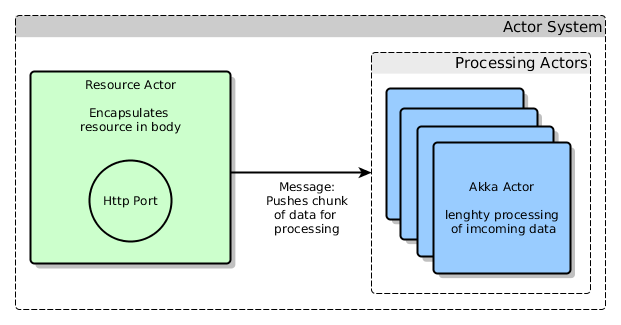
\includegraphics[scale=0.4]{figures/akkaExample1.png}
	\caption{Simple arrangements of actors}
	\label{fig:akkaExample1}
\end{figure}

As seen in figure \ref{fig:akkaExample1} the resource is encapsulated by an actor and not directly accessible from the outside. The Resource actor has sole access to the resource and internally buffers data. The actors which want to process the incoming data need to be known to the Resource so that it can push the incoming work to the processing actors. The source actor will try to find a free actor for the input and then send a message containing the data to it. If there is no free worker, it will buffer the data. Keep in mind that details needed for a functioning implementation are left out, this is a mere demonstration of the design principles used.

But already there are some properties of this construct which are worthwhile to point out: Actors will not block a thread when there is no work to be done. Only when the source distributes work, the workers will come alive and start doing things, instead of busy waiting or blocking on the source. The system is event-driven which can drastically streamline processing in an application that is dependent on input from outside clients.

Failure is another important aspect of an actor system. If a task which a worker is performing crashes due to an unexpected error in the processing of data, i.e. an error while parsing a data-structure from the input String the worker will terminate. One principle of Akka concurrency is rather than explicitly handling every  possible exception,to just let the actor crash. In this case it will send a termination message containing the error to its parent and/or supervising actor. 
The responding supervisor can then decide whether the actor should resume working using the next message in its mailbox, be restarted, or stopped altogether.
In Akka (and Erlang) this is called the \textit{Error Kernel Pattern} which means that delicate tasks which might crash are delegated to disposable actors which carry no crucial data. Crashing in these actors can even be expected behavior upon certain input.

Now for the example, the processing actors could be supervised by the data-source itself, which would decide what to do if one actor crashes. Or this role could be assigned to a designated supervisor actor such that the source and the processing workers live independently and the supervisor with its children act similar to a threadpool (See Figure \ref{fig:akkaExample2}).

\begin{figure}[h]		
 	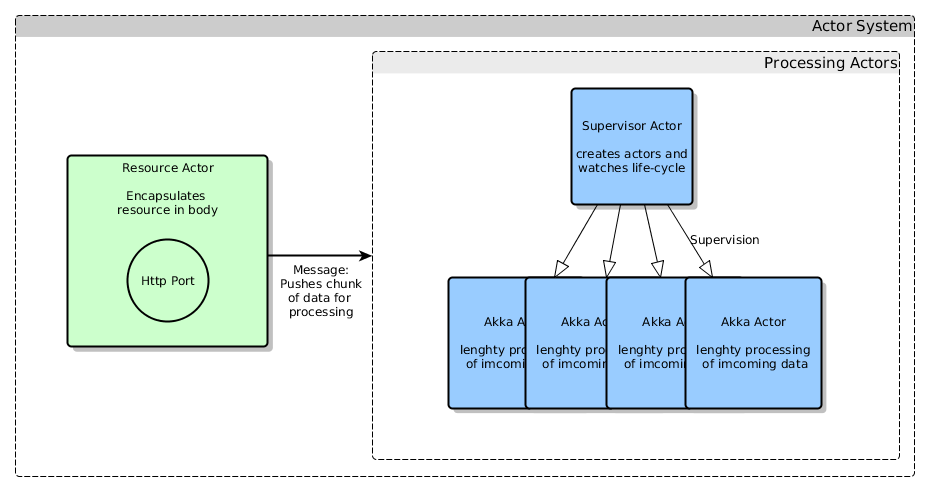
\includegraphics[scale=0.4]{figures/akkaExample2.png}
	\caption{Arrangement of actors with supervision}
	\label{fig:akkaExample2}
\end{figure}

This very flexible model for concurrency allows for the modeling of complex data-flows in large systems. Using supervision and messaging most software patterns such as producer/consumer scenarios or divide and conquer can be implemented elegantly without race conditions, busy waiting, or excessive spawning of threads. Akka was shown to produce some impressive performance figures on large-scala systems. In fall 2013 a cluster of 2400 nodes was run on Google Compute Engine which shows how well scaling out via remoting is possible \cite{link:akkaCluster}. Also it is possible to scale up quite drastically. One benchmark shows how a single machine throughputs around 50 million messages a second in a tuned out system \cite{link:akkaScaleUp}. The machine used though is very powerful with 48 cores and 128GB RAM (one of the biggest Amazon EC2 machines, the r3.4xlarge, has 16 cores and 122GB RAM in comparison) \cite{link:ec2Pricing}.


Akka is - all in all - a very powerful and flexible tool which provides the possibility to scale in all dimensions. It is a complex tool with quite some overhead for the implementation. But once this is overcome, it is an excellent tool to scale a system without having to restructure the code too much. Also it makes for elegant and readable code.


\subsubsection{Spray}
The Spray toolkit has been developed since 2011 \cite{link:sprayChangelog} and has more than 50 contributors so far \cite{link:sprayGithub}. The prescribed goal was to create a powerful, flexible and fast HTTP-Server for Scala which works well with other packages and applications and follows good practices for Scala code which have developed so far.\\

Most important aspects include:\\
\begin{itemize}
	\item HTTP-server implementation with high-level interface.
	\item High throughput using Akka, various error-handling already in place.
	\item Flexible in deployment, works well with actor-systems.
\end{itemize}

Having to expose the functionalities of the database to clients over TCP/IP is one of the very basic requirements.
Technically Akka gives a developer all the tools to write an actor sitting on top of the port, buffering input and flexibly distributing workload over all available processing workers (see the example figure \ref{fig:akkaExample2}). But this requires for quite some work to fulfil all the requirements of HTTP for timeouts, errors, status reports and many more.

Spray implements most of this behavior already out of the box in a fashion similar to the examples given in Section \ref{sec:akka}.
Fundamentally Spray is built on top of Akka to provide largely parallel, non-blocking and resilient web-applications. 
The developer has all the handles needed to tune his the frontend of his application according to the needs of the application.

Spray handles all incoming requests and boxes them in case classes. The developer then implements how to distribute the incoming requests to actors by providing a listening actor. The receiving actors contain the processing logics and send back the result after completion. The result is then automatically formatted back to an Http-response. In case or errors Spray responds with meaningful error messages and handles time-out strategies, which can be adjusted in configuration.

Being an Akka-based toolkit scaling the system follows the same principles as Akka's, meaning that large systems can be build without the need for rewriting the logics.

Note that for Scala there exists also the \textit{Play Framework} to create a webb-application on-top of scala code, which is very well maintained \cite{link:play}. 
It offers the developer a complete HTTP server with easy to use routing. But Play is optimized for RESTful web-apps made to be read by humans. It does not offer options to decide on how exactly incoming requests are dispatched to an Akka actor system. The overhead is therefore too big and the focus too far away from the requirements of the task at hand, where clients are in most cases other programs which take care of rendering the information for the user.


\subsubsection{Blueprints-API}
Blueprint API offers a framework which enables a flexible integration of the database to the system by abstracting over details of database implementations.

\begin{itemize}
	\item Class hierarchy for \textit{Graph-Databases}.
	\item Abstracts away the underlying implementation of the graph.
	\item Offers a domain specific language for queries against graphs and other toolkits.
\end{itemize}
 
It is central to the database system to be able to perform efficiently on graph databases. The Blueprint API lets the developer chose the level of abstraction he wants have over the actual implementation used for the graph (see \cite{link:blueprints} for more information). 
The idea of Blueprints is to provide a complete hierarchy of classes and interfaces to support multiple underlying databases without the need to change higher-level code. This allows for a meaningful distinction of low-level code from higher-level code in the system. The actors which would handle requests to the database use the API on a higher level while optimization and efficient algorithms can be developed in depth closer to the database implementation.
There are many implementations of the Blueprints API including the MongoDB based MongoDBGraph an OrientDB implementation called OrientDBGraph and Titan Graph database.
The API also offers supplementary utilities for graphs such as a toolkit for algorithms (Furnace), an DSL for traversals (Gremlin) and tools for dataflow processing (Pipes) which can greatly reduce the need to write redundant code.


\subsubsection{Titan Database}
Titan Database is an implementation of the Blueprints interface developed since 2012 and builds the functionality of a graph database conforming to the Blueprints API  using variable backends. Its highlights include:

\begin{itemize}
	\item Scalability for graphs.
	\item Efficient complex graph traversal.
	\item Atomicity, Consistency, Isolation, Durability (ACID).
	\item Seamless integration of indexing backends.
\end{itemize}
(s.o. \cite{link:titanHome} for further information).

Supported backends include Cassandra, HBase and most interestingly Oracle Berkeley DB. The latter allows for fast prototyping in memory without the need to handle a large database in which keys have to be created, dropped and recreated upon necessary adjustments of the data schemas \cite{link:berkeleyDB}. It is in itself already capable to accommodate 10-100 million vertices on decent hardware \cite{link:titanWithBerkeley}. As indexing backends Elastic Search and Apache Lucene are supported.

The ability to change the backend and connecting to existing databases is powerful during development. Prototyping can be realised with lightweight databases and then for production a large more independent database can be used making changes mostly in the configuration alone. This implies that the database  could eventually even live on another machine altogether if scaling requires it. Together with Blueprint's abilities this ensures that that code for prototyping can be  reused in production later without many changes in the logic of the code. Scaling benefits from this structure, too. 

Titan makes full use of the Blueprints syntax to iterate over the graph and thus enables a rich existing toolkit to be used.
Having the indexing backends integrated makes optimization of queries possible and allows to extract the full abilities of the graph structure of the database in comparison to relational systems.

\subsubsection{Elastic Search}
Elastic Search is one of the possible indexing-backends which can be combined with Titan DB. 

\begin{itemize}
	\item Fast-growing popular indexing software.
	\item Supported by Titan DB.
	\item Fast, powerful and flexible.
	\item Allows for search in large systems.
	\item Used in companies for huge data-sets.
\end{itemize}

Indexing the graph database is very important since nodes are normally retrieved using parent nodes and subsequently descending into the graph. For example if a client wants to retrieve a function with a specific name the system would retrieve the general function node and iterate over \textit{all} child-nodes. This is a linear operation which will be costly once the system reaches a reasonable size and thus introduces a large toll on the most important task: searching the database for functions and their implementations. Indexing can then allow fast access to elements via creation of keys over nodes. Later the indices could also be used to power a search-engine for parts of text in the documentation or parts of source-code itself.
Elastic search is open source and was founded in 2012 and has since seen dramatic growth. Just recently it received a \$70 million round C-funding while having around half a million downloads of their software a month. \cite{link:esAbout} \cite{link:esTechCrunch} I is used in today's big-data contexts to power meaningful search over largely unstructured data in near real-time. 
I
ndices generated in the graph could even be used to monitor performance in the system such as frequencies of transactions, update-times, number of users and many more in real-time. Elastic Search should be part of the design right from the beginning because of the vast potential in usages later while introducing little overhead for the initial design.

It is a powerful tool to create queryable indices on a multitude of data sources. It allows for quick context dependent search, completion and scoping of queries and fast access to elements in the database.
Some applications which use Elastic Search on a big scale include Github, SoundCloud and Yelp!. These companies use the software over terrabytes of data and billions of datapoints. \cite{link:esUses}
	
%%%%%%%%%%%%%%%%%%%%%%%%%%%%%%%%%%%%%%%%%
\subsection{First Sketch - Design of my Implementation}
\label{sec:firstSketch}
%%%%%%%%%%%%%%%%%%%%%%%%%%%%%%%%%%%%%%%%%
In this section the first Prototype will be described regarding its setup and interplay of different parts of the software. It is demonstrated which tasks are handled and how requests are answered.

\begin{figure}[h!]		
 	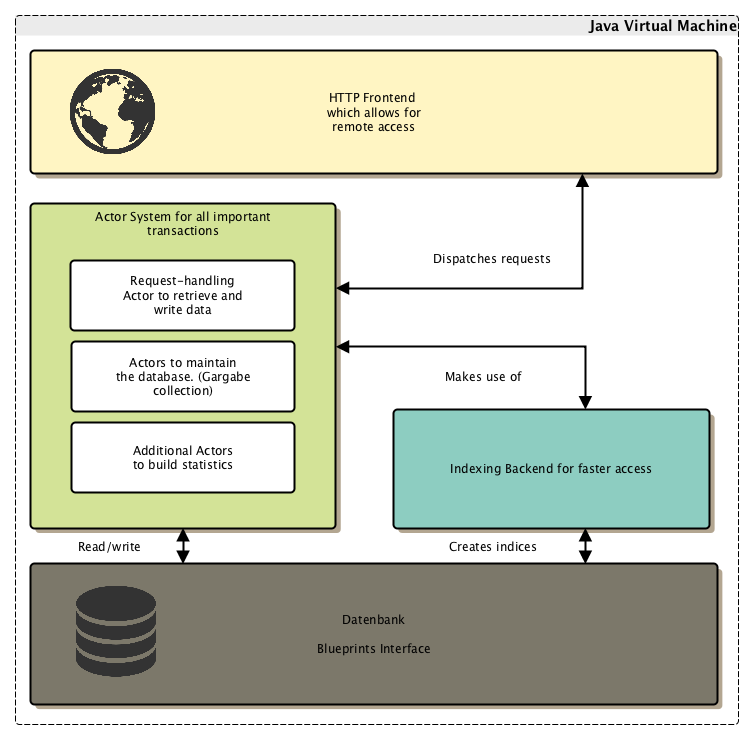
\includegraphics[scale=0.5]{figures/roughOverview.png}
	\caption{Overview over the system}
	\label{fig:roughOverview}
\end{figure}

\subsubsection{Elements of the Design}
% Rough overview
Bringing all the  tools mentioned in \ref{sec:softwarePackages} together the initial design sketch has several parts to consider as seen in figure \ref{fig:roughOverview}

\begin{enumerate}
	\item The Database in which data are stored and retrieved from.
	\item An indexing backend which reads the database and creates the indices for fast access.
	\item A system of Akka-actors which can work on the database in serveral ways:
	\begin{enumerate}
		\item To write and retrieve things to and from the database.
		\item To maintain the database.
		\item To build statistics on the available data.		
	\end{enumerate}	
	\item An HTTP 'frontend' which offers the handles to the functionality of the database to the outside world.
\end{enumerate}

A general principle for the first sketch is to run as much as possible in the same JVM to enhance inner-process speed and make the configuration more straightforward by not having several different settings for all the different parts of the system. This also speeds up the startup procedure and centralizes logging for faster analysis when things do go wrong in the initial prototypes. \\

\textbf{1. The Database}\\
The initial backend to which provides the graph structure is Titan Database configured for decent parallel access. As a storage backend  BerkeleyDB in-memory database is used which keeps the data used for queries on the heap which of course will only work for rather small databases. But it is easy to setup and works well on home-sized machines. The testing-server is a low-energy optimized machine with a tiny dual-core processor the rather memory-focused approach helps achieving moderate testing performance. As stated in the Titan Documentation (\cite{link:titanWithBerkeley}) this database is capable of holding millions of nodes and edges and is thus sufficient for the early testing of the storing schemes. 
The database itself already allows for parallel access. Therefore the database is used without any changes to the interface. 
Due to the Blueprint Interface all the code written against the Titan-Database-backend could be run on other databases without any actual changes to the code at all, if necessary. The variables are settings in the configuration for the application to allow connection to the remote JVM which runs the database.
Building on this foundation should allow for meaningful tests which can give good predictions of the performance of a more elaborate setup and also show bottlenecks and errors very early.\\

\textbf{2. The Indexing Backend}\\
Elastic Search can be embedded into the Berkeley Database with the disadvantage, that it will only be accessible from the same JVM. For the first prototype this does not cause problems since everything is supposed to run in the same virtual machine.
The indices have to be created when keys are introduced to the database to allow for fast incremental indexing.

TODO LIST over what I plan to index and how this index can be used for faster retrieval and/or search.	\\

\textbf{3. The Actor System to Do the Processing}\\	
The single most important and interesting part of the system is the Akka actor system with its various functions for the database. This is the part where the online system really begins to come alive since it offers the processing powers to enhance the system above the functionality of a simple remotely accessed database or a version control system. 
Initially there are three classes of functions a)-c) to be distinguished:\\

a)A set of actors which exists to process incoming requests from \textit{users} of the database. \\

This level of the  program should abstract away from different databases and their details in implementation, so that the frontend can access a clean interface to interact with the data.
Principally there is an architecture of classes for the actors in place in which only the lowest level of actors has to adapt to the details of the database implementation used. General functionality such as supervision, behavior on timeout, handling of wrong queries and the communication with the frontend is handled higher up in the architecture.This has the following effects:

Behavior of the system can be tested and reasoned over on a higher level, boilerplate code is minimized and actors become interchangeable depending on the backend which is in place. Potentially, actors could be switched \textit{on runtime} to adapt to situations in the system. For example there could be one actor which handles reads and writes but when the database is overloaded, actors  which refuse to do some computationally expensive tasks will be put in place. Having this structure allows for very fine-grained control over the handling of requests. Actors can react to small changes themselves but could also be switched altogether when there exist significant problems.
Akka actors are pretty lightweight (since they do not represent a thread) and are thus cheap to create and destruct. The first Implementation makes use of this fact as such that a new worker is spawned for every incoming connection to the database. It will then handle all communication from the user to the  backend  and once the connection is shut down it will silently die and release all its resources. Of course this reasoning is based on a hypothetical world where no problems with garbage collection exist in the JVM. This could be a potential bottleneck to the system. One way to overcome this would be to make use of actor-pools instead of dynamically spawning them and destroying them after (a possibly very) brief lifetime.
As a general design principle one can see the separation of implementation of processing-functions and behavior. An actor implementation should describe the \textit{what} rather than the \textit{how} of connection handling. For example this includes how to connect a user, how to funnel his request to the database, retrieve the results and send them back. This is why actors are to carry as little of actual parsing, database or number-crunching code, but rather call static objects which contain the implementation. It is very easy to exchange implementations for different databases without refactoring any of the code used inside the actors. Handling connections is closely connected to the Spray and thus will be explained in the upcoming paragraph on the frontend.\\

b) Garbage collection in the database\\
One of the upcoming challenges for the database is cluttering because of the very open structure for writing to the database.
There might be thousands of implementations for one method or a user decided to make unnecessarily many versions of his code.
The database should be able to reduce quantity on some levels. For example it could remove older versions of code which were not used for a very long time, index only recent versions, delete unpopular code or compact things which have not been used for some time.
The idea here is to iterate over parts of the database which were not maintained for some time and iterate over the produced statistics and use decision rules what to remove. The first design will focus only on the most important things and will most likely not incorporate any of the above named.\\

c) Creating statistics on the database\\
This is were the inherent properties of a graph database really come into play. Iterating over existing functions and the collected metrics such as usage counts, usage dates, number of distinct users, number of implementations and many basic metrics more to create meaningful higher level statistics. This could include recommendation of code based on concepts such as code complexity, amount of dependencies, speed, memory-efficiency and so forth. These workers are supposed to work quite similar to the garbage collection in that they can be spawned depending on how much capacity there is and then do independent runs on subbranches of the database without corrupting the state of other parts. Those workers will have to do quite expensive computations and will therefore be a hallmark in testing the capability of the system. In the end these actors will have to work quite close to the database used and at this point an exact scheme of abstraction does not seem helpful.\\

\textbf{4. The Frontend to Open the System to the Outside World}\\
The Spray framework is used for this task as explained earlier in \ref{sec:softwarePackages}. 
Following is a description of the basic principles of Spray and how they are used in the system.
Spray has a configured port on which the application listens which is encapsulated by a dispatching actor. This actor extends a Spray class which provides an interface for the  HTTP transfer and leaves the implemtation of the dispatching of requests to the user. This means that the port is free again quickly, together with HTTP tunneling requests are consumed fast. The dispatcher buffers the incoming requests and then distributes the workload over other actors. Initially it creates a new actor which will process the task at hand. One useful  aspect of Spray is that every actor which takes an incoming request from the dispatcher implicitly knows where to send back the computed response to without seeing any of it in the code. Also the dispatcher knows about the actor processing the request and will send an adequate error message back to the user on failure such as a timeout or a complete crash of an actor. This way error handling becomes quite elegant and effortless since the handling actors do not need to implement any of it in most cases. Their crashing should give enough information to the dispatcher. Once the dispatcher knows about problems in the backend it could change dispatching strategies or dispatch a different kind of handling-actors altogether.

Everything after dispatching a request to a handling actor happens asynchronously and non-blockingly. The actor depends on nothing but his own local state, reading or writing from or to the database and then returning the response once it is done working. There is no timing needed, no waiting on things and thus the chance for serious deadlocks or race conditions is pretty low.

One interesting aspect for the first sketch is the fact that the actor-system created for Spray is used for all the actors handling requests to the database. This may be a bit brittle in the long run but works fine in the short run since the actors are created by Spray and are thus "nearby" with no remote handling needed. Also these actors form a necessary unit with the HTTP server. One does not make sense without the other.

\begin{figure}[h!]		
 	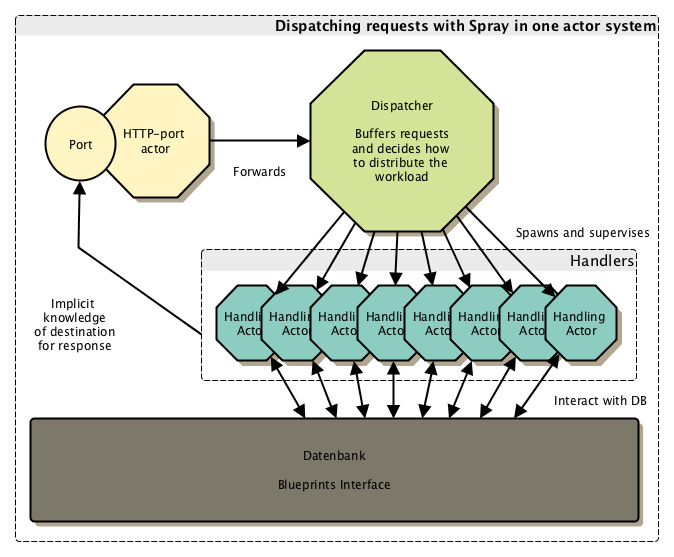
\includegraphics[scale=0.6]{figures/sprayDispatcher.png}
	\caption{How the Dispatcher distributes requests}
	\label{fig:sprayDispatcher}
\end{figure}

\subsubsection{Database Schema}
The term database schema must not be confused with what it means in 'classical' relational databases (as for example in chapter three of \cite{fundamentalsDatabase}). Here it  means the structure of nodes and edges in combination with fields within the two. Nevertheless this schema must be designed well since it will determine what kind of tasks can be accomplished quickly and satisfactorily to the user. The schema will be explained exemplary instead of giving an all-engrossing explanation of the schema to show the underlying ideas rather than listing all details of the implementation. Also having a graph database means that the structure is sometimes best explained by figures instead of text.\\

First of all the graph should have different entry points to traverse the elements in order  to extract data in a meaningful context. Traversals will also be used to create the statistics later on. Figure \ref{fig:dbStructure1} shows how this structure is built for the central storage unit of Julia functions. Most of the tree are meta-nodes which do not contain any code but define the place of the code. The code itself then resides in the leafs (which are a specific version of a method's implementation).  The meta-structure is crucial to the database since this is the part where the graph structure really comes into play separating it from a relational database (which would contain the leafs in tables).

\begin{figure}[h!]		
	\floatbox[{\capbeside\thisfloatsetup{capbesideposition={right,top},capbesidewidth=6cm}}]{figure}[\FBwidth]
	{\caption{The general organization for functions in the database. There is a function node which is parent to all function nodes which represent only names for functions (corresponding to symbols in Julia). Depicted here is one specific Function A with all its subtrees, leaving out all the other possible functions. The children of a function are the multiply dispatched methods which have a unique signature. The next deeper level are different implementations for one method (possibly by different users or focusing on different aspects) and then finally the leafs containing all the code, documentation and other (meta-)data are called version (at different time points). Having this structure alows for traversals to find all methods for a function or any of the version for any of the implementation using straightforward graph-syntax from the Blueprints interface.}\label{fig:dbStructure1}}
	{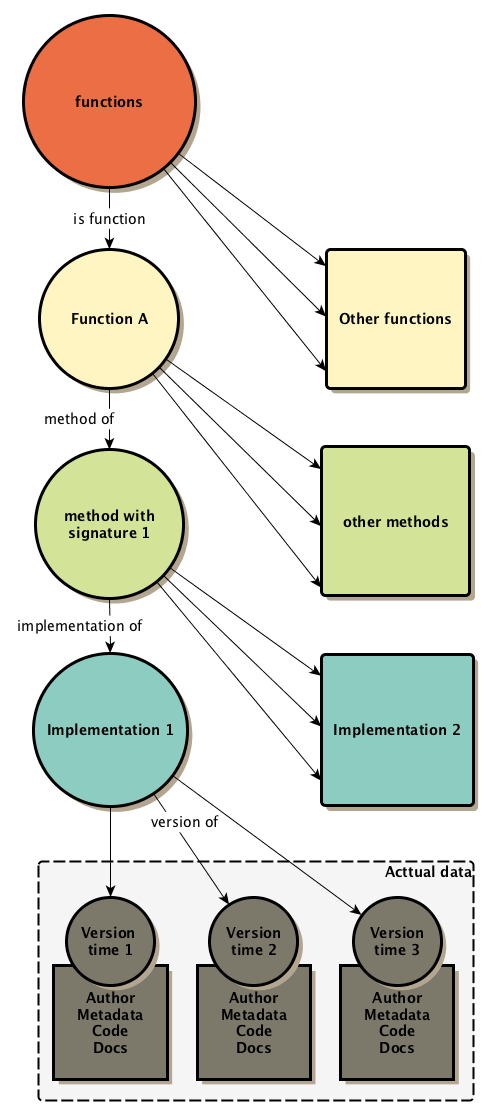
\includegraphics[width=8cm]{figures/dbStructure1}}
\end{figure}

Extending this structure to yield more entry points and possibilities for traversals is depicted in figure \ref{fig:dbStructure2}. Datastructures to link Julia types to where they are used in arguments and a draft to declare dependencies in the graph are introduced. Note that this structure does not alter the functions themselves, but just adds more nodes and edges. In reality with Titan Databases it is possible to add structure later on without the need to reload data. This might come in very handy when trying to extend functionality of the system.

\begin{figure}[h!]		
 	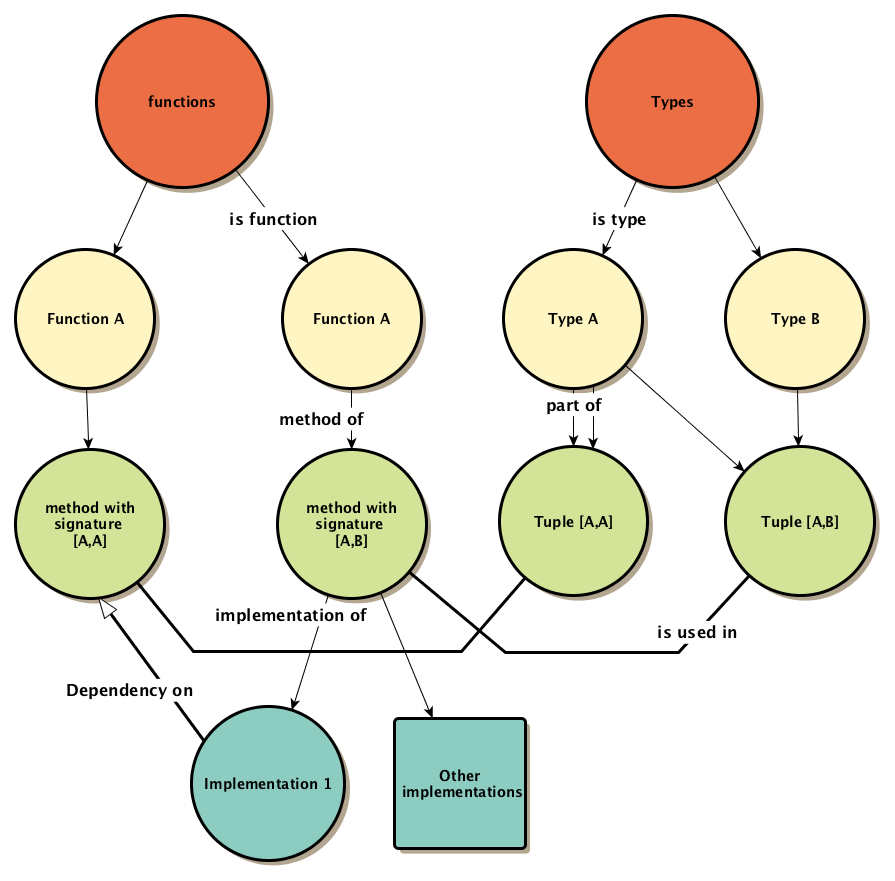
\includegraphics[scale=0.4]{figures/dbStructure2.png}
	\caption{Added structures in the database.}
	\label{fig:dbStructure2}
\end{figure}

Statistical data is incorporated into the meta-structure and the leaf nodes themselves. Usage counts, sets of users, last updates, ratings, complexity, speed or memory consumption and any other metric imaginable can be stored for different methods of functions and also for different implementations of one method.

\subsubsection{The HTTP-Protocol}
Central from a user's point of view is the access to the system. The program should be client agnostic and therefore  HTTP is a good interface because its structure closely matches the desired functionality of the program. HTTP is supposed to be restful (which is not always the case) which helps modeling a database-connection.

Users can do GET requests to retrieve data, including specifications of parameters in the header and even pieces of code in the body of a request. Insertions into the database can be modeled via POST requests. 

HTTP then offers many error codes when things go wrong. From timing out to temporary unavailability there are lot of messages which are well documented and used in thousands of websites and thus well-known to most programmers who want to create a client to the system.

--- TODO  genaue Struktur erst klar, wenn Tests gemacht wurden ---
--- TODO Referenz auf Fundamentals of Database Systems p. 63 - "Three-schema-architecture" ---



\subsection{A deeper look into the implementation - for those interested}
All actors carry most of the implementation code in their companion object instead of the class itself to decouple implementations of logics from those of behavior. The cake pattern \cite{link:cakePattern} makes it possible to implement much of the connection handling in the trait HandlerActor without any code to handle a database.  An instance of DbHandlerActor is then used with an instance of the trait DbInteractions. This trait mixes in the needed details to connect to a specific database. Using this pattern the system is very flexible to incorporate different databases or changes to implementation without disturbing other parts of the system. To be continued...

\begin{figure}[h!]		
 	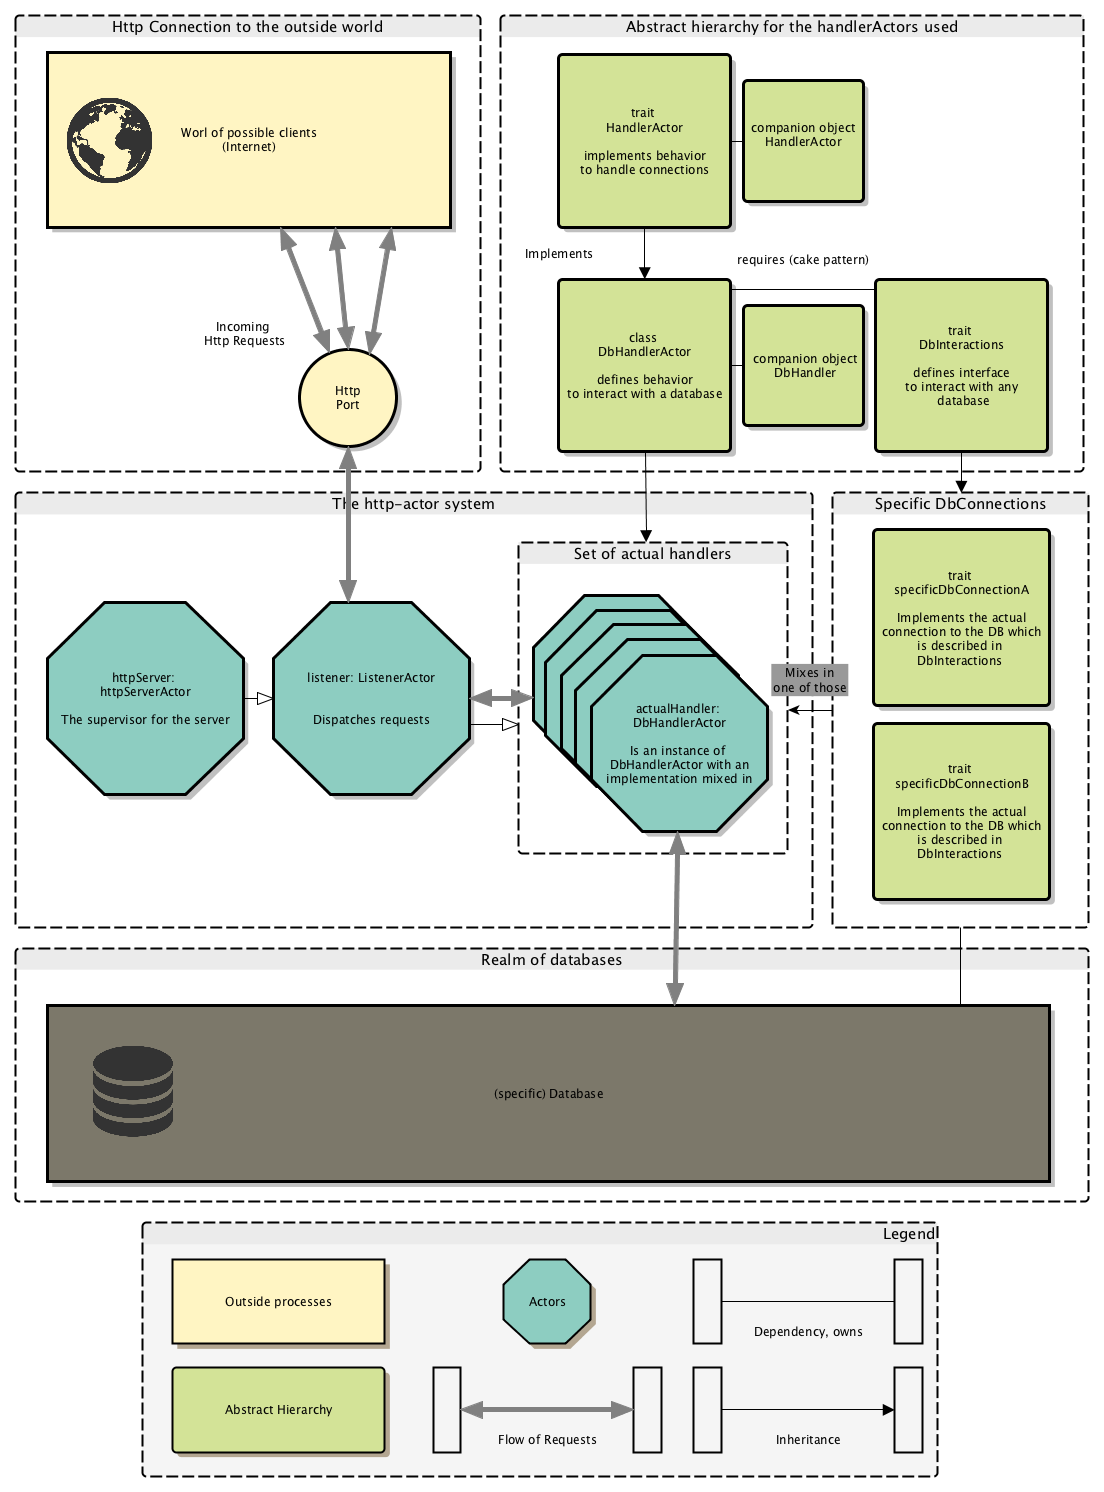
\includegraphics[scale=0.35]{figures/requestFlow.png}
	\caption{Detailed view of the system and how requests are handled. }
	\label{fig:requestFlow}
\end{figure}

\subsection{Evaluation of the First Sketch}
\subsection{Description of the Iteration}
\subsection{Further Evaluation}




%%%%%%%%%%%%%%%%%%%%%%%%%%%%%%%%%%%%%%%%%%%%%%%%%%%%%%%
% Conclusions
\section{Conclusions}
\label{sec:conclusions}
%%%%%%%%%%%%%%%%%%%%%%%%%%%%%%%%%%%%%%%%%%%%%%%%%%%%%%%
\subsection{State of the Implementation at the End of My Work}
\subsection{Comparison to Requirements and Goals}
What was fulfilled, what not and what might be critical. Can the application be extended? What have I achieved at what can people to with it at the time?\\
%\textcolor{red}{Is the code I wrote usable from the clients perspective?}
\subsection{What to Come - Future from here on}
What are the next steps and which people can get involved. How do I see the chances in the future. Concluding thoughts on performance and scalability.
\subsection{Summary}


%%%%%%%%%%%%%%%%%%%%%%%%%%%%%%%%%%%%%%%%%%%%%%%%%%%%%%%
% Appendix
%%%%%%%%%%%%%%%%%%%%%%%%%%%%%%%%%%%%%%%%%%%%%%%%%%%%%%%
\section*{Appendix A - References}
%%%%%%% Bibliographie %%%%%%%%%
\bibliography{sources}
\bibliographystyle{plain}

\end{document}